\documentclass[a4paper,11pt,twoside,openright]{book}


\usepackage[utf8]{inputenc}
%\usepackage[vietnam.english]{babel}

\usepackage[T1]{fontenc}




%\usepackage[Latin1]{inputenc}       %caractËres accentuÈs et autres
%\usepackage[T1]{fontenc}            %cÈsure des mots accentuÈs
%\usepackage[frenchb]{babel}         %francisation (chapitre,annexe,rÈfÈrences...)
\usepackage{graphicx}               %insertion graphiques

\usepackage{a4wide}
%\usepackage{psfig}


%\psfigurepath{}




%\usepackage{times}


%\input{transfig}



\renewcommand{\thefootnote}{}

%% Necessaire pour creer les index
\usepackage{makeidx}
\makeindex





%%%%%%%%%%%%%%%%%%%%%%%%%%%%%%
%%%% MODIFY THIS PART FOR THE FIRST PAGE

% change the master level 
\def\MasterLevel{Master Thesis }
%\def\MasterLevel{Master 1}

\def\InternshipTitle{[Title of internship]}
\def\FirstName{Khoa}
\def\LastName{Nguyen Nhu}
\def\HostOrganization{ICTLab-USTH}
\def\CityName{Hanoi}
\def\CountryName{Vietnam}
\def\UniversityName{[University name]}
\def\Supervisor{Dr. Tran Giang Son}



\setlength{\textwidth}{175mm}
%
\setlength{\textheight}{245mm}

\setlength{\topmargin}{-10mm}

\setlength{\evensidemargin}{-8mm}

\setlength{\oddsidemargin}{-8mm}

% ----------------------- DEBUT DOCUMENT ---------------------------

\begin{document}



\pagestyle{plain}



\pagenumbering{Roman}


% ----------------- DEFINITION DU TITRE ET DES AUTEURS ---------------------------

\newpage
\empty
\thispagestyle{empty}

\begin{center}




%\includegraphics[angle=0,width=5cm]{images/usth-logo-final-transparent.png}



\includegraphics[angle=0,width=5cm]{logo-1_39.png}


\vspace*{1cm} 



{\huge University of Science and Technology of Hanoi }\\


\vspace*{1cm} 


{\large Information and Communication Technology Department}\\


\vspace*{1cm} 



{\huge \MasterLevel }\\


\vspace*{1cm} 

{\large Academic year 2016 -  2017}


\vfill


\noindent\hrulefill

\vspace*{2mm} 

{\Large \InternshipTitle }


\noindent\hrulefill





\vfill 



{\large presented by } \\

\vspace*{5mm} 


{\large \bf \FirstName~  \LastName} \\


\vspace*{5mm} 


%{\large registered at \UniversityName } \\



%\vspace*{5mm} 



{\large supervised by  \Supervisor } \\


\vspace*{20mm} 




{\large Host organization :   \HostOrganization }


\vspace*{5mm} 


{\large  \CityName~- \CountryName} \\

\vspace*{5mm} 





%\noindent\hrulefill


\end{center}


% ----------------------- PAGE VIDE ---------------------------




\chapter*{ATTESTATION}



\vfill


\noindent\hrulefill

~\\


I hereby,  \FirstName~  \LastName, certify that my report doesn't contain plagiarism (copy/paste) from other sources.

~\\

In case of plagiarism in my report, I know the consequences and I understand that my report won't be evaluated. In this case, my M1 internship will be noted as "fail".


~\\

 Date 

~\\
 
 Signature 
 ~\\

 \FirstName~  \LastName
 

~\\
~\\
~\\
~\\
~\\

\noindent\hrulefill


\vfill


\vfill



%\selectlanguage{vietnam}
%
%
%Tôi ký tên dưới đây, <họ> <tên>, xác nhận rằng bài báo cáo của tôi không có đạo văn (lỗi sao chép) từ các nguồn khác.
%
%
%~\\
%
%
%Nếu bị phát hiện ra trong bài báo cáo, tôi biết hậu quả và tôi hiểu rằng bài báo cáo của tôi sẽ không được chấp nhận. 
%Trong trường hợp đó, học phần (thực tập năm thứ nhất, thực tập năm thứ hai, hay học phần đánh giá) sẽ bị ghi là “không đạt”.
%
%
%
%~\\
% 
%Ngày … tháng … năm …
% 
%
%~\\
% 
%Chữ ký
%
%
%~\\
%~\\
%~\\
%
%
%\selectlanguage{english}
%
%\noindent\hrulefill




\setcounter{page}{1}



% ----------------------- ACKNOWLEDGEMENTS ---------------------------

\chapter*{Acknowledgements}

First and foremost, I would like to express my deepest gratitude to Dr. Tran Giang Son, my research supervisor for his patience, helpful theoretical and practical advice and enthusiastic encouragement during the period of my internship. \\
Second, I am grateful for all the support along the internship period of Assoc. Prof. Ngo Duc Thanh and Assoc. Prof. Damien Gratadour\\
Also, I want to thank the University of Science and Technology of Hanoi (USTH) in general and specifically, the USTH ICTLab for granting me this opportunity to work as one of the temporary member of the lab. \\
Last but not least, I would like to appreciate the support from my family and friends during my internship. \\





% ----------------------- RESUME ---------------------------


\chapter*{Asbtract}

In recent years, parallel computing has become more popular, with the advancement of hardware, such as multicore processor, and the development of parallel architecture. Nowadays, parallization exists in many places, such as modern day PC/Workstation, Cluster, Grid Computing system or High Performance Computing system in general. This is due the demand for enhancement in computing performance to solve enormous, complex problem. \\
The main focus of the intership is to investigate potential improvement for the Regional Climate Model with GPU and parallelization, and provide some proofs of concept for this matter. Testing will be conducted using OpenMP Parallel API.\\
~\\
Keyword: Parallel Computing, OpenMP, Regional Climate Model, High Perfomance Computing

% ----------------------- PAGE VIDE ---------------------------


% ----------------------- REMERCIEMENTS ---------------------------

%\include{Thanks}

% ----------------------- TABLE DES MATIERES ---------------------------



\tableofcontents{}


\newpage


\listoffigures{}

\newpage

\listoftables


\newpage



\chapter*{List of Abreviations}


\newpage




% ----------------------- TABLE DES FIGURES ---------------------------
%\listoffigures{}

% ----------------------- TABLE DES TABLES ---------------------------
%\listoftables{}

% ----------------------- TABLE DES TABLES ---------------------------
%\listoflistings{}

% ----------------------- CHAPITRE ---------------------------
\pagenumbering{arabic}

\chapter{Introduction}

\section{Context and Motivation}

Climate models are representations of factors that have impacts on climate, described by mathematical equations based on the law of physics. Main factors that can affect the climate are the atmosphere, oceans, living creatures, land exterior, ice, and energy produced by the Sun. Together with other sophisticated elements such as cloud, rainfall, water evaporation, etc., these climate models are put into use in order to achieve various objectives such as studying the tendencies of climate systems or estimating future climate ~\cite{climate_modeling}. Not only incoming energy emitted from the sun, as mentioned above, is taken into consideration in the form of short-wave electromagnetic radiation, but also outgoing long-wave infrared electromagnetic one. With both of these radations are taken into account, any changes that cause imbalance between the two will result in a change in temperature, thus changing the climate. ~\cite{jana_majumder_2011}. \\
~\\
Climate models, with the way their data and computations are processed, have benefited greatly from exploiting parallelism, especially with vector processors and the recently extended Single Instruction Multiple Data parallel paradigm. However, most of the climate models today are computed in cluster-based computer with large, powerful microprocessors, which are unable to fully utilize parallelism to a greater extent. This is due to the fact that CPUs lack the necessary memory bandwidth to obtain such level of parallelism, no matter how powerful the CPU can be.\\
~\\
University of Science and Technology of Hanoi (USTH) research lab REMOSAT, led by Assoc. Prof Ngo Duc Thanh, has been in urgent need for perfomance boost and computation time acceleration of the climate models running in the lab, specifically, the Regional Climate Model system, or RegCM for short. In this context, the goal of the internship is to investigate possible usage of GPU in climate models simulation performed by the REMOSAT research lab to speed up its processing time.\\

\section{Regional Climate Model system (RegCM)}

The Regional Climate Model system, also known as RegCM, unlike other global climate models, was developed using Fortran as a limited area model for the purpose of long term simulation in specific regions. RegCM is meant to be used as a public, open source software that is user-friendly and portable enough to be apply in any domains in the world. Being a community model, and is designed to be applied in a vast number of communities, RegCM has partaken in a large number of regional climate projects, and has been aiding various climate studies and future climate predictions ~\cite{regcm_man}. \\
~\\
Originally created by the National Center of Atmospheric Research (NCAR) back in 1989, it has now evolved over time after numerous of patches and a few major updates. As of the most recent release, RegCM4, the program contains many upgrades and new features compare to previous versions. Most noticably, RegCM has now improved on flexibility, portablity and user friendliness, and is now fully supported by the Earth Physics System, as the developers commented in the Documentation ~\cite{regcm_ictp}. \\
~\\
A typical run of Regional Climate Model system consists of two main parts. First, based on the global dataset, the system will generate input data for the simulation, including the domain of simulation, sea surface temparature, initial condition, boundary condition, and other optional dataset ~\cite{regcm_man}. After being successfully produced, these input data are put in the RegCM program to run the simulation. It is worth mentioning that RegCM supports Open Message Passing Interface(OpenMPI), which is a standard API for parallel/distributed computing built on the Message Passing parallel model. Upon completing, the program will generate output models of the simulation, containing information on atmosphere status, surface diagnostic variables, radiation fluxes, and a save point that holds the model's status at the end of the run, which enables the simulation to restart at that point, thus allowing the user to split a long simulation into much many shorter ones. \\

\section{Limitation of RegCM}

While having full OpenMPI support, meaning that it can run simulation in parallel using the Message Passing parallel paradigm, RegCM still has some limitations in its parallelism. First and foremost, since the method of implementing parallelization is OpenMPI, CPU-based parallelism is utilize while running simulations, which imply the above mention restriction about lack of memory bandwidth, especially when parallel processes need to exchange data with each other. Moreover, CPU parallelization limits the number of processes can run simutaneously to no more than the number of logical cores the CPU has, which can hurt the performance on lower core count CPUs. Another drawback that the developers have pointed out regarding RegCM's parallel implementation is that it current has no form of parallel I/O, indicate that not all processes can have access to the data at the same time ~\cite{regcm_man}. \\

\section{Host Institution}

ICTLab of University of Science and Technology of Hanoi (USTH) is a joint international research laboratory in the field of Information and Communication Technology (ICT) between USTH and other French partners. The lab has researchers from USTH, Institute of Information Technology (IOIT) of Vietnam Academy of Science and Technology (VAST), Institut de Recherche pour le Dévelopment (IRD) and the University of La Rochelle, France ~\cite{ictlab}. \\
~\\
\begin{figure}[h]
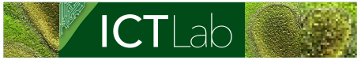
\includegraphics[angle=0,width=10cm]{ictlab_logo.png}
\centering
\caption{ICTLab Official Logo}
\end{figure}
~\\
The ICTLab was created on December 1st, 2014, supported by USTH, French Embassy in Vietnam, 13 French high education institutes and universities (namely, USTH Consortium), and the Asian Development Bank (ADB) ~\cite{ictlab}. \\
~\\
The researches of ICTLab focus on two main applicative axes: Cultural heritage preservation and promotion, and Environmental protection and Environmental risk management. Fundamental research programs target common scientific activities, such as Modeling, Image Processing and Analysis, Machine Learning, Expert User Interaction, Geographical Information Systems, Information Retrieval, and Sensor ~\cite{ictlab}. \\
~\\
Regarding to these research activities, ICTLab is currently working on two main projects. The first project, SWARMS (Say and Watch: Automated image/sound Recognition for Mobile monitoring Systems), aims to achieve a flexible and real-time monitoring network, where device can used as both passive sensors and active transmitter that can send visual, voice, textual pieces of information to a monitoring system, so that stakeholder can analyze and forecast information. The other project, ARCHIVES (Analysis and Reconstruction of Catastrophes in History within Interactive Virtual Environments and Simulations), focuses on supporting historical research on past disasters with assistance of advance document image processing and analysis, information retrieval, machine learning, Geographical Information System (GIS) representation and agent-based computer modeling ~\cite{ictlab}. \\

\section{Thesis organization}

The thesis is organized as follow. Excluding the first chapter, which is Introduction, there are 4 chapters. The \nth{2} chapter discusses about background knowledge related to general paralellization, local parallelism and high performance computing. Chapter 3 explains the methodology carried out during the internship period. Testing and result are shown in the \nth{4} chapter, and the last chapter will conclude the thesis with remarks, limitation and possible future works. 






% ----------------------- CHAPITRE ---------------------------

\include{StateOfTheArt}

% ----------------------- CHAPITRE ---------------------------

\include{Contribution}

% ----------------------- CHAPITRE ---------------------------

\chapter{Results}


This part must contain the result of the method/algoritm/system developed during the internship. \\

This part must also include comparisons with the state of the art.\\

Use tables, figures, graphics to illustrate your results. \\ 

Comment your results, and explain the context used to obtain these results.







% ----------------------- CHAPITRE ---------------------------

\chapter{Conclusion}


You can recall the problematic of your internship and explain if you have solved all the problem or not. \\

Recall the methods used and your contribution.\\

Recall the results obtained and explain the quality of your results in comparison with the state of the art.\\


Give some perspectives of your work.



% ----------------------- BIBLIOGRAPHIE ---------------------------

\bibliography{Biblio}
\bibliographystyle{unsrt}

% ----------------------- ANNEXES ---------------------------

\appendix

\appendix

\chapter{Detail about ...}

In this part, you can add more details about some technical parts which need too much detailed impossible to include in the report body of your report








\chapter{Mathematical demonstration}

If necessary, you can add appendix to show mathematical demonstrations.





\end{document}
